%-------------------------------------------------------------------------------
%                                PREAMBLE
%-------------------------------------------------------------------------------
\documentclass[usenames,dvipsnames,svgnames,10pt,aspectratio=169]{beamer}
%
\usefonttheme{professionalfonts}
% This theme uses TIKZ: compile twice with PDFLaTeX or LuaLaTeX.
%
%  Options:
%  - [clean]:    clean slides, i.e. logos and footbar are removed
%  - [kth]:      footbar style inspierd to the official KTH template
%  - [nicewave]: a different style of wave is used (not approved by FLOW)
%
\usetheme[clean]{flow}

\usepackage{tikz}
\usetikzlibrary{arrows}
\usetikzlibrary{shapes.geometric, math, positioning, calc, patterns, angles, quotes}
\usetikzlibrary{patterns.meta,decorations.pathmorphing}

\newcommand{\semaphore}[3]{% #1: color of circle,
                           % #2: color of semicircle
                           % #3: angle of semicircle 
  \tikz[node distance=0mm,baseline]
       {
         \node (s1) [circle, fill=#1, minimum size=6mm] {};
         \node      [semicircle, fill=#2, 
           inner sep=0pt, outer sep=0pt, minimum size=3mm,
           anchor=south,
           at={(s1.center)}, rotate=#3] {};
       }
}

\usepackage[]{circuitikz}

\usepackage{pgfplots}
\usepgfplotslibrary{polar}

\usepackage{hyperref,graphicx,lmodern}
\usepackage[utf8]{inputenc}
\usepackage{media9}
\usepackage{xcolor}
\usepackage{stmaryrd}
\usepackage{nicefrac}
\usepackage{multimedia}
\usepackage{multicol}
\usepackage{upgreek}
\usepackage[]{bm}
\usepackage[]{url}
\usepackage[]{animate}
\usepackage{amsmath}

\graphicspath{{imgs/}}
\setbeamertemplate{blocks}[rounded][shadow=true]

\DeclareMathOperator*{\maximize}{maximize~}

%-------------------------------------------------------------------------------
%                                TITLE PAGE
%-------------------------------------------------------------------------------
\title[Nonlinear physics] % Short title used in footline
{
	Limit cycles cannot exist
}

\author[J.-Ch.~Loiseau] % Presenting author in short form used in footline
{
	\underline{Jean-Christophe Loiseau}
}
% - Give the names in the same order as the appear in the paper.
% - Underline the presenting author.

\institute[unused]
{
	\url{jean-christophe.loiseau@ensam.eu} \\
	Laboratoire DynFluid \\
	Arts et M\'etiers, France.
}
% Keep it simple, no one is interested in your street address.

% University logo(s)
\logot{
\includegraphics[width=.128\paperwidth]{DynFluid_logo}}  % Top logo
\logob{
\includegraphics[width=0.128\paperwidth]{ENSAM_logo}} % Bottom logo
% \logoc[{\includegraphics[width=.128\paperwidth]{limsi}}]{\includegraphics[width=.128\paperwidth]{limsi}} % Corner logo
%
% Cover image: \cvrimg{x position}{y position}{cover image}
\cvrimg{.77}{.8}{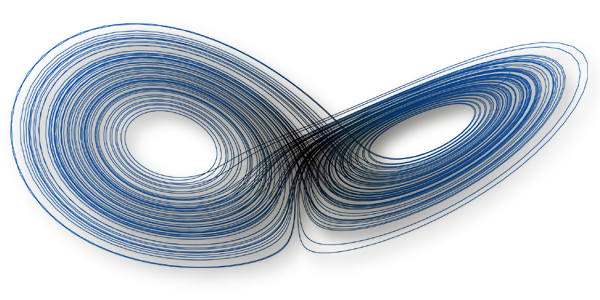
\includegraphics[width=.4\paperwidth]{cover.png}}

\date[unused]{Physique non-lin\'eaire -- 2019-2020}

\begin{document}

\titleframe	% Print the title as the first slide

%-------------------------------------------------------------------------------
%                           PRESENTATION SLIDES
%-------------------------------------------------------------------------------

\begin{frame}[t, c]{Limit cycles}{}
  \centering
  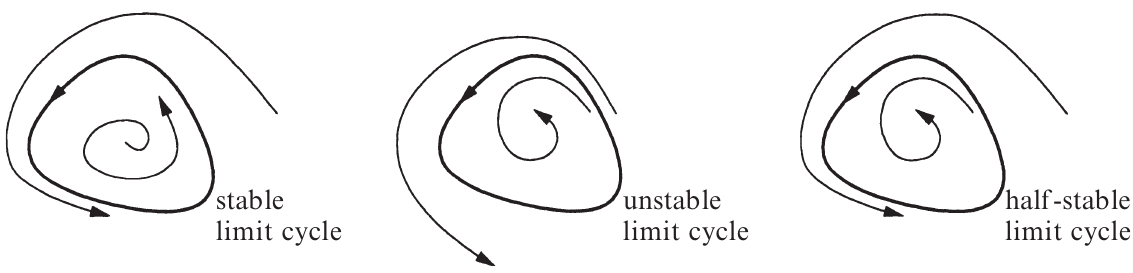
\includegraphics[width=.8\textwidth]{limit_cycles}
  \vspace{1cm}
\end{frame}

\begin{frame}[t, c]{Closed orbits are not always limit cycles!}{}
  \begin{minipage}{.6\textwidth}
    Linear systems $\dot{\bm{x}} = \bm{Ax}$ can have periodic solutions if $\textrm{eig}(\bm{A}) = \pm i \omega$.
    They are not limit cycles though.
    If $\bm{x}(t)$ is a periodic solution, so is $\alpha \bm{x}(t) \quad \forall \alpha \neq 0$.
    These closed orbits are not \alert{\textbf{isolated}}.
  \end{minipage}%
  \hfill
  \begin{minipage}{.36\textwidth}
    \centering
    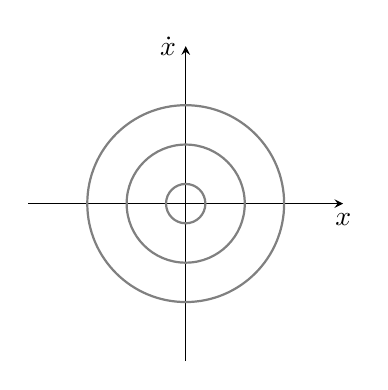
\begin{tikzpicture}[>=stealth]
      \draw[->] (-2, 0) -- (2, 0) node[below] {$x$};
      \draw[->] (0, -2) -- (0, 2) node[left] {$\dot{x}$};

      \draw[->, gray, thick] (0, 0) circle (0.25) node[] {};
      \draw[->, gray, thick] (0, 0) circle (0.75) node[] {};
      \draw[->, gray, thick] (0, 0) circle (1.25) node[] {};
    \end{tikzpicture}
  \end{minipage}
\end{frame}

\begin{frame}[t, c]{Limit cycles at not always circle in phase space}{}
  \begin{minipage}{.48\textwidth}
    \centering
    \textbf{van der Pol oscillator}

    \[
    \ddot{x} + \mu \left( x^2 - 1 \right) \dot{x} + x = 0
    \]
  \end{minipage}%
  \hfill
  \begin{minipage}{.48\textwidth}
    \centering
    \begin{tikzpicture}[>=stealth]
      \draw[->] (-2, 0) -- (2, 0) node[below] {$x$};
      \draw[->] (0, -2) -- (0, 2) node[left] {$\dot{x}$};

      \draw[gray, smooth, thick] plot file{van_der_pol_traj_9.txt};
    \end{tikzpicture}
  \end{minipage}
\end{frame}

\begin{frame}
  \vfill
  \centering
  \Large
  When are periodic dynamics \alert{\textbf{impossible}}?
  \vspace{-1cm}
  \vfill
\end{frame}

\begin{frame}[t, c]{Gradient systems}{}
  \begin{minipage}{.48\textwidth}
    Consider the single-valued scalar function $V(\bm{x})$ such that the system we consider can be written as
    %
    \[
    \dot{\bm{x}} = -\nabla V(\bm{x}).
    \]
    %
    This is a \alert{\textbf{gradient system}} with \alert{\textbf{potential function}} $V(\bm{x})$.
  \end{minipage}%
  \hfill
  \begin{minipage}{.48\textwidth}
    \centering
    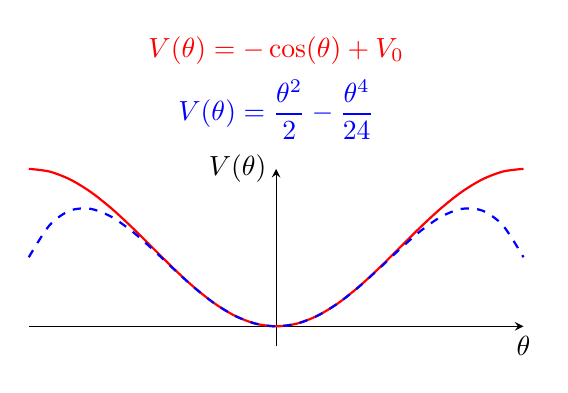
\begin{tikzpicture}[>=stealth]
      \draw[->] (-pi, 0) -- (pi, 0) node[below] {$\theta$};
      \draw[->] (0, -0.25) -- (0, 2) node[left] {$V(\theta)$};

      \draw[red, domain=-pi:pi, variable=\x, thick, smooth] plot (\x, {-cos(\x r) + 1}) {};
      \draw[blue, dashed, domain=-pi:pi, variable=\x, thick, smooth] plot (\x, {0.5 * \x * \x - (1/24)*(\x)^4}) {};

      \node[red] at (0, 3.5) {$V(\theta) = -\cos(\theta) + V_0$};
      \node[blue] at (0, 2.75) {$V(\theta) = \dfrac{\theta^2}{2} - \dfrac{\theta^4}{24}$};
    \end{tikzpicture}
  \end{minipage}
\end{frame}


\begin{frame}[t, c]{Gradient systems}{}
  \begin{minipage}{.48\textwidth}
    \centering
    \textbf{Theorem:} Closed orbits are impossible in gradient systems.
  \end{minipage}%
  \hfill
  \begin{minipage}{.48\textwidth}
    \centering
    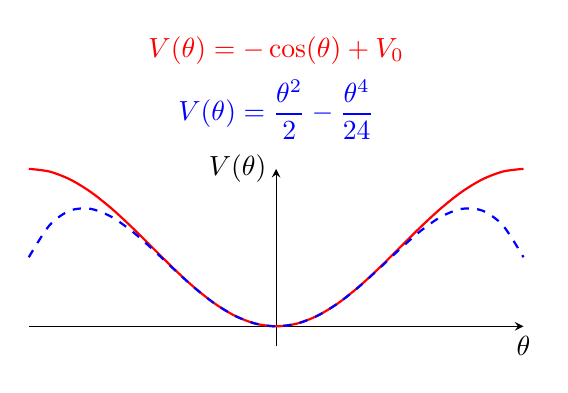
\begin{tikzpicture}[>=stealth]
      \draw[->] (-pi, 0) -- (pi, 0) node[below] {$\theta$};
      \draw[->] (0, -0.25) -- (0, 2) node[left] {$V(\theta)$};

      \draw[red, domain=-pi:pi, variable=\x, thick, smooth] plot (\x, {-cos(\x r) + 1}) {};
      \draw[blue, dashed, domain=-pi:pi, variable=\x, thick, smooth] plot (\x, {0.5 * \x * \x - (1/24)*(\x)^4}) {};

      \node[red] at (0, 3.5) {$V(\theta) = -\cos(\theta) + V_0$};
      \node[blue] at (0, 2.75) {$V(\theta) = \dfrac{\theta^2}{2} - \dfrac{\theta^4}{24}$};
    \end{tikzpicture}
  \end{minipage}
\end{frame}

\frame{}

\begin{frame}[t, c]{Lyapunov functions}{}
  \begin{minipage}{.68\textwidth}
    It is sometimes possible to construct an energy-like function that decreases along trajectories.
    This is known as a \alert{\textbf{Lyapunov function}}.
  \end{minipage}%
  \hfill
  \begin{minipage}{.28\textwidth}
    \centering
    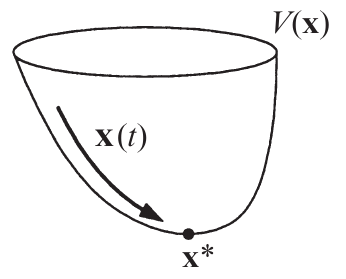
\includegraphics[width=\textwidth]{lyapunov}
  \end{minipage}
\end{frame}


\begin{frame}[t, c]{Lyapunov functions}{}
  \begin{minipage}{.68\textwidth}
    Consider a system $\dot{\bm{x}} = f(\bm{x})$ with a fixed point at $\bm{x}^*$.
    A \alert{\textbf{Lyapunov function}} $V(\bm{x}) : \mathbb{R}^n \to \mathbb{R}$ needs to satisfy the following properties
    %
    \begin{enumerate}
    \item It is continuously differentiable.
    \item $V(\bm{x}) > 0$ for all $\bm{x} \neq \bm{x}^*$ and $V(\bm{x}^*) = 0$.
    \item $\dot{V} < 0$ for all $\bm{x} \neq \bm{x}^*$.
    \end{enumerate}
    %
    If such a function function exists, $\bm{x}^*$ is globally asymptotically stable.
  \end{minipage}%
  \hfill
  \begin{minipage}{.28\textwidth}
    \centering
    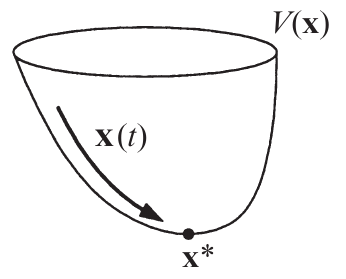
\includegraphics[width=\textwidth]{lyapunov}
  \end{minipage}
\end{frame}

\frame{}

\begin{frame}[t, c]{Dulac's criterion}{}
  \begin{minipage}{.68\textwidth}
    Let $\dot{\bm{x}} = f(\bm{x})$ be a continuously differentiable vector field defined on a simply connected subset $R$ of the plane.
    If there exists a continuously differentiable function $g : \mathbb{R}^2 \to \mathbb{R}$ such that $\nabla \cdot \left( g \dot{\bm{x}} \right)$ has one sign throughout $R$, then there are no closed orbits lying entirely in $R$.
  \end{minipage}%
  \hfill
  \begin{minipage}{.28\textwidth}
    \centering
    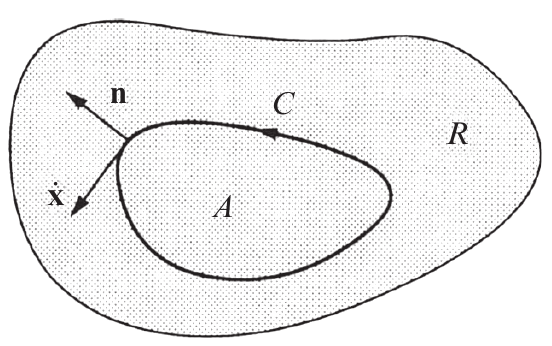
\includegraphics[width=\textwidth]{dulac}
  \end{minipage}
\end{frame}

\frame{}

\begin{frame}[t, c]{Divine inspiration}{}
  \begin{minipage}{.68\textwidth}
    Checking if the system is a \alert{\textbf{gradient system}} is relatively simple.
    Unfortunately, there is no systematic way to construct \alert{\textbf{Lyapunov functions}} or the $g(\bm{x})$ function in \alert{\textbf{Dulac's criterion}}.
    If you can find such functions for your problem, these are however very powerful results.
  \end{minipage}%
  \hfill
  \begin{minipage}{.28\textwidth}
    \centering
    
\includegraphics[width=.8\textwidth]{idea}
  \end{minipage}
\end{frame}

\end{document}
